\documentclass[letterpaper, 10 pt, conference]{ieeeconf} 

\IEEEoverridecommandlockouts                            
\overrideIEEEmargins
\makeatletter
\let\NAT@parse\undefined
\makeatother

\usepackage[dvipsnames]{xcolor}

\newcommand*\linkcolours{ForestGreen}

\usepackage[utf8]{inputenc}
\usepackage[T1]{fontenc}
\usepackage[brazilian]{babel}
\usepackage{times}
\usepackage{graphicx}
\usepackage{amssymb}
\usepackage{gensymb}
\usepackage{amsmath}
\usepackage{breakurl}
\def\UrlBreaks{\do\/\do-}
\usepackage{url,hyperref}
\hypersetup{
colorlinks,
linkcolor=\linkcolours,
citecolor=\linkcolours,
filecolor=\linkcolours,
urlcolor=\linkcolours}

\usepackage{algorithm}
\usepackage{algorithmic}

\usepackage[labelfont={bf},font=small]{caption}
\usepackage[none]{hyphenat}

\usepackage{mathtools, cuted}

\usepackage[noadjust, nobreak]{cite}
\def\citepunct{,\,} 

\usepackage{tabularx}
\usepackage{amsmath}

\usepackage{float}

\usepackage{pifont}
\newcommand{\cmark}{\ding{51}}%
\newcommand{\xmark}{\ding{55}}%

\newcommand*\diff{\mathop{}\!\mathrm{d}}
\newcommand*\Diff[1]{\mathop{}\!\mathrm{d^#1}}
\newcommand*\imgres{600}

\newcommand*\GitHubLoc{https://github.com/Reis25/FenomenoDosTransportes}

\newcolumntype{Y}{>{\centering\arraybackslash}X}

%\usepackage{parskip}

\usepackage[]{placeins}

\newcommand\extraspace{3pt}

\usepackage{placeins}

\usepackage{tikz}
\newcommand*\circled[1]{\tikz[baseline=(char.base)]{
            \node[shape=circle,draw,inner sep=0.8pt] (char) {#1};}}
            
\usepackage[framemethod=tikz]{mdframed}

\usepackage{afterpage}

\usepackage{stfloats}

\usepackage{atbegshi}
\newcommand{\handlethispage}{}
\newcommand{\discardpagesfromhere}{\let\handlethispage\AtBeginShipoutDiscard}
\newcommand{\keeppagesfromhere}{\let\handlethispage\relax}
\AtBeginShipout{\handlethispage}

\usepackage{comment}
\newcommand{\estiloR}{
  \lstset{ %
    language=R,                     % the language of the code
    basicstyle=\footnotesize,       % the size of the fonts that are used for the code
    numbers=left,                   % where to put the line-numbers
    numberstyle=\tiny\color{gray},  % the style that is used for the line-numbers
    stepnumber=1,                   % the step between two line-numbers. If it's 1, each line
                                    % will be numbered
    numbersep=5pt,                  % how far the line-numbers are from the code
    backgroundcolor=\color{white},  % choose the background color. You must add \usepackage{color}
    showspaces=false,               % show spaces adding particular underscores
    showstringspaces=false,         % underline spaces within strings
    showtabs=false,                 % show tabs within strings adding particular underscores
    frame=single,                   % adds a frame around the code
    rulecolor=\color{black},        % if not set, the frame-color may be changed on line-breaks within not-black text (e.g. commens (green here))
    tabsize=2,                      % sets default tabsize to 2 spaces
    captionpos=b,                   % sets the caption-position to bottom
    breaklines=true,                % sets automatic line breaking
    breakatwhitespace=false,        % sets if automatic breaks should only happen at whitespace
    title=\lstname,                 % show the filename of files included with \lstinputlisting;
                                    % also try caption instead of title
    keywordstyle=\color{blue},      % keyword style
    commentstyle=\color{darkgreen},   % comment style
    stringstyle=\color{red},      % string literal style
    escapeinside={\%*}{*)},         % if you want to add a comment within your code
    morekeywords={*,...}          % if you want to add more keywords to the set
}}

\usepackage{xcolor}
% Definindo novas cores
\definecolor{verde}{rgb}{0.25,0.5,0.35}
\definecolor{jpurple}{rgb}{0.5,0,0.35}
\definecolor{darkgreen}{rgb}{0.0, 0.2, 0.13}
%\definecolor{oldmauve}{rgb}{0.4, 0.19, 0.28}
% Configurando layout para mostrar codigos Java
\usepackage{listings}


\title{\LARGE \bf
High-Performance Scientific Computing Case Study
}

\author{Demétrios Reis Costa$^{1}$% <-this % stops a space
\thanks{$^{1}$Demétrios é graduando na universidade federal de Alagoas, cursa engenharia da computação.
Email: demetriosreis@ic.ufal.br}%
}


\begin{document}


\maketitle
\thispagestyle{empty}
\pagestyle{empty}


%%%%%%%%%%%%%%%%%%%%%%%%%%%%%%%%%%%%%%%%%%%%%%%%%%%%%%%%%%%%%%%%%%%%%%%%%%%%%%%%
\begin{abstract}

This article provides a practical overview of numerical solutions to the heat equation using the finite difference method. The heat equation that we’ll model is important in many scientific fields. In mathematics, the prototypical parabolic partial differential equation can be used to describe a wide variety of time-dependent phenomena, including heat conduction, particle diffusion, and ocean acoustic propagation. A direct practical application of the heat equation, in conjunction with Fourier theory The heat equation that we’ll model is important in many scientific fields. In mathematics, the prototypical parabolic partial differential equation can be used to describe a wide variety of time-dependent phenomena, including heat conduction, particle diffusion, and ocean acoustic propagation. A direct practical application of the heat equation, in conjunction with Fourier theory.

\end{abstract}

%%%%%%%%%%%%%%%%%%%%%%%%%%%%%%%%%%%%%%%%%%%%%%%%%%%%%%%%%%%%%%%%%%%%%%%%%%%%%%%%
\section{INTRODUÇÃO}

Esse trabalho visa analisar uma simulação natural de fenômenos naturais em modelam problemas naturais, mais especificamente
estamos interessados na modelagem das equações que descrevem o calor. Traduzida matematicamente da seguinte forma:

\begin{equation*} \frac{\partial\phi}{\partial t}=\alpha\frac{\partial^{2}\phi}{\partial x^{2}},\tag{1} \end{equation*}

Segundo Eysenck: "Modelagem computacional é uma área de conhecimento multidisciplinar que trata da aplicação de modelos matemáticos e técnicas da computação à análise, 
compreensão e estudo da fenomenologia de problemas complexos em áreas tão abrangentes quanto as engenharias, ciências exatas, biológicas, humanas, economia e ciências 
ambientais".\\
Sendo assim notamos o caráter multidisciplinar que somos submetidos ao estudarmos e detalharmos a natureza da equação de 
calor sob um determinado recurso computacional. 
Os modelos de simulação permitem decisões facilitadas em sistemas caracterizados por elevado número de variáveis, além de  reduzirem os custos da implementação em si do sistema 
em questão. Nota-se que as modificações como por exemplo, nos recursos produtivos de um sistema podendo ser: adição de novas máquinas, identificação dos gargalos produtivos ou 
até mesmo redução de tempos de processo. \\
Esse último item é o foco do presente trabalho onde analisaremos a performance computacional das máquinas frente utilização da modelagem e simulação das equações de calor. 
Algumas métricas são pré-estabelecidas e dadas pelo artigo que seguiremos \textit{The Heat Equation: High-Performance Scientific Computing Case Study}, e nele há questionamentos 
(5), dos quais as respostas nortearão o conteúdo, bem como as discussões e resultados.  A princípio esperamos que o sistema comporte-se de forma eficiente a medida que a paralelização de processo seja maior. Em 
suma esperamos:
\begin{itemize}
    \item Redução do tempo de execução relativa ao aumento de processadores;
    \item Possibilidade de inferir melhorias em partes do sistema bem como dotá-lo  da capacidade de expansão; 
    \item Redução do tempo de execução de experimentos através da divisão do modelo de simulação entre os processadores;
    \item Aumento do grau de tolerância à falha,ou mesmo analisar caso as diretivas tratem esse problema automaticamente. 
\end{itemize}

%%%%%%%%%%%%%%%%%%%%%%%%%%%%%%%%%%%%%%%%%%%%%%%%%%%%%%%%%%%%%%%%%%%%%%%%%%%%%%%%
\section{Metodologia}

A modelagem matemática por finalidade a descrição de um fenômeno natural através de equações consistentes dotadas de 
sentido físico e similar, podendo ser observada e medida. No entanto nem sempre é simples analisar e medir sistemas 
naturais pelo número de interações (ciclos de processo) que precisamos fazer, o que implica em um alto consumo 
computacional. 
O relatório em questão segue uma metodologia correlata ao artigo que estamos analisando, não sendo um problema uma vez que 
o trabalho contribui com: \\

\begin{itemize}
    \item Definição e delimitação do problema;
    \item Modelagem de sistema;
    \item Métricas de avaliação;
    \item Ferramentas e tecnologias de software.\\
\end{itemize}
	Sendo o trabalho do autor:
\begin{itemize}
    \item Averiguação da performance do sistema trabalhando com sistemas distribuídos;
    \item Comparações e explicações de resultados.\\
\end{itemize}

Na abordagem geral notamos que teremos uma abordagem top-down é adotada nessa etapa. Onde iremos  analisar a fundamentação 
matemática e computacional, os problemas de compilação e gestão de recursos computacionais serão abstraídos pelo openMP, 
uma biblioteca a seguir melhor explicada. O uso das diretivas do OPENMP implicam que as transições que representam a 
chamada de método não estarão em conflito com outras transições e pela natureza do nosso sistema temos também que as 
transições associadas à chamada de método são sempre instantâneas.
Em suma temos uma metodologia clássica usada nesse tipo de trabalho:

\begin{figure}[htbp]
\centering
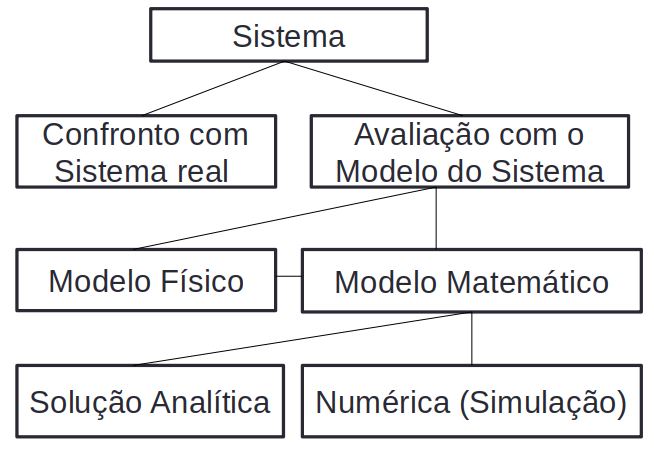
\includegraphics[width=0.97\columnwidth]{Figuras/img1.png}
\caption{Fluxo de métodos seguido.}
\label{stability}
\end{figure}

Essa abordagem foi proposta por Law e Kelton (2000), nota-se que iremos nos deter na última etapa do método referente. 
%%%%%%%%%%%%%%%%%%%%%%%%%%%%%%%%%%%%%%%%%%%%%%%%%%%%%%%%%%%%%%%%%%%%%%%%%%%%%%%%
\section{Tecnologias}

Entendemos tecnologia como: Teoria ou análise organizada das técnicas, procedimentos, métodos, regras, âmbitos ou campos da ação humana. É nesse sentido que encaramos os  algoritmos como uma tecnologia que pode ser avaliada na nossa medição.
Segundo (TOSCANI, 2001) deve-se projetar um algoritmo de modo que  seja o melhor possível, garantindo bom desempenho e integridade. Existem vários critérios de avaliação de um 
algoritmo como: quantidade de trabalho requerido, quantidade de espaço requerido, simplicidade, exatidão de resposta e otimalidade. Complexidade refere-se à complexidade de tempo
de execução de cálculos em uma máquina de Turing multi fita (que é uma  máquina comum com várias fitas).  Pelo modelo fornecido no artigo os modelos de algoritmos que usamos não 
são ótimos. A Fim de reproduzir as análises devem ser levados em consideração tomando como base a tabela (1)

\begin{table*}[!hbt]
%\centering
\begin{tabular}{|c|c|c|c|c|}
	\hline
	Operação  & Entrada & Saída & Algoritmo & Complexidade \\
	\hline\hline
	Matriz de multiplicação & M =(n*m)*(m*p) & matriz n*p & & O(n3) \\
	\hline
	Matriz de multiplicação & M =(n*m)*(m*p) & matriz n*p &2 de Strassen & O($n^{2.807}$)\\
	\hline
	Matriz de multiplicação & M =(n*m)*(m*p) & matriz n*p & de Coppersmith–Winograd & O(n$^{2.376}$) \\
	\hline
	Matriz de multiplicação & M =(n*m)*(m*p) & matriz n*p &6 CW-like otimizado &O(n$^{2.376}$)\\
	\hline
	Matriz de multiplicação &  M =(n*m)*(m*p) & matriz n*p &83.33 &O(n$^{2.376}$)\\
	\hline
	Matriz de inversão & M =(n*m)*(m*p) & & Eliminação de Gauss–Jordan &O(n$^{2.376}$)\\
	\hline
	Matriz de inversão & M =(n*n)  & M =(n*n) & de Strassen &O(n$^{2.376}$)\\
	\hline
	Matriz de inversão & M =(n*n)  & M =(n*n) & de Coppersmith–Winograd & O(n$^{2.376}$)\\
	\hline
	Matriz de inversão & M =(n*n) & M =(n*n) & CW-like otimizado & O(n$^{2.376}$) \\
	\hline
	Adição & Dois números de n dígitos &  número de n + 1 dígitos & & \Θ(n)\\
	\hline
	Subtração & Dois números com n dígitos  & número de n + 1 dígitos & & \Θ(n)\\
	\hline
	Multiplicação & Dois números com n dígitos & número com 2n dígitos &  & O(n2)\\
	\hline
	Multiplicação & Dois números com n dígitos & número com 2n dígitos & Algoritmo Karatsuba & O(n$^3$)\\
	\hline
	Multiplicação & Dois números com n dígitos & número com 2n dígitos & de Toom–Cook & O(n$^3$)\\
	\hline
	Multiplicação & Dois números com n dígitos & número com 2n dígitos & k-forma de Toom–Cook & O(nlog (2k − 1)/log k)\\
	\hline
	Multiplicação & Dois números com n dígitos & número com 2n dígitos & Toom–Cook (Knuth 4.3.3-T) & O(n 2\sqrt{2} log n log n)\\
	\hline
	Multiplicação & Dois números com n dígitos & número com 2n dígitos & Schönhage–Strassen & O(n log n log log n)\\
	\hline
	Multiplicação & Dois números com n dígitos & número com 2n dígitos &  de Fürer & O(n*og(n)*2O(log*n))\\
	\hline
\end{tabular}
\caption{Complexidade dos algoritmos.}
\label{t1}
\end{table*}
Por causa da possibilidade de por blocos inverter uma matriz, onde uma inversão de uma n*n 
matriz requer inversão de duas
matrizes com metade do tamanho e seis multiplicações entre duas matrizes com metade do 
tamanho, e uma vez que a 
multiplicação de matrizes tenha um limite inferior de \Ω ( n 2 Predefinição:Var log) 
operações, pode ser demonstrado que o 
algoritmo de dividir e conquistar que usa a inversão por blocos para inverter uma matriz é 
executado com a mesma 
complexidade de tempo que o algoritmo de multiplicação de matrizes que é usado internament.

\begin{itemize}
    \item openMP
\end{itemize}
O OpenMP (do inglês Open Multi-Processing, ou Multi-processamento aberto) é uma interface 
de programação de aplicativo(API)
para a programação multi-processo de memória compartilhada em múltiplas plataformas. 
Permite acrescentar simultaneidade aos
programas escritos em C, C++ e Fortran sobre a base do modelo de execução fork-join.
É constituída por um conjunto de diretivas de compilador, rotinas de biblioteca, e 
variáveis de ambiente que influenciam o 
comportamento do tempo de execução, como é explicitado na figura (2).
\begin{figure}[htbp]
\centering
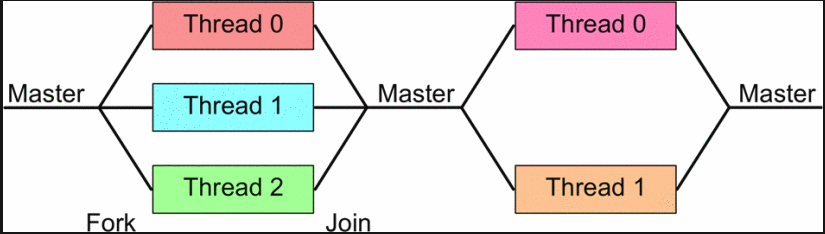
\includegraphics[width=0.97\columnwidth]{Figuras/img2.png}
\caption{Esquema de fluxo de dados OPENMP.}
\label{stability}
\end{figure}
Nota-se que a noção de gestão do hardware é melhorada e o usuário deve preocupar-se apenas com a sincronização da disponibilidade de recursos 
Definido em conjunto por um grupo principal de fornecedores de hardware e de software, o OpenMP é um modelo de programação portável e escalável que proporciona aos programadores 
uma interface simples e flexível para o desenvolvimento de aplicações paralelas para as plataformas que vão dos computadores de escritório até os supercomputadores. 

\begin{itemize}
    \item Especificações \textbf{openMP}:
    \item Package: libomp-dev
\item Version: 5.0.1-1
\item Priority: extra
\item Section: universe/libdevel
\item Source: openmprtl
\item Origin: Ubuntu
\item Maintainer: Ubuntu Developers
\item Original-Maintainer: LLVM Packaging 
\item Bugs: https://bugs.launchpad.net/ubuntu/+filebug
\item Installed-Size: 29,7 kB
\item Depends: libomp5 (= 5.0.1-1)
\item Suggests: libomp-doc
\item Breaks: libiomp-dev (<< 3.7-1)
\item Replaces: libiomp-dev (<< 3.7-1)
\item Homepage: http://openmp.llvm.org/
\item Supported: 3y
\item Download-Size: 5.088 B
\item APT-Manual-Installed: yes
\item Description: LLVM OpenMP runtime - dev package
 \item while it is executing.
\end{itemize}

\\
\begin{itemize}
    \item Compilador: \textbf{GCC}; 
\end{itemize}

\begin{itemize}
    \item Linguagens usadas: \textbf{C} e \textbf{Matla}.
\end{itemize}
\begin{itemize}
    \item Sistema operacional: \textbf{Linux}:  Linux demetriosreis 4.18.0-25-generic #26~18.04.1-Ubuntu SMP Thu Jun 27 07:28:31 UTC 2019 x86\_64 x86\_64 x86\_64 GNU/Linux
;
\end{itemize}


Hardware:


%%%%%%%%%%%%%%%%%%%%%%%%%%%%%%%%%%%%%%%%%%%%%%%%%%%%%%%%%%%%%%%%%%%%%%%%%%%
\section{Métricas}

[botar aqui a def do paper]
A motivação do presente relatório é a constatação da eficiência do uso de um método computacional paralelo, nisso
usamos mais de um núcleos disponível para alcançar a solução para o nosso problema. Idealmente, devemos chegar à solução 
para o mesmo problemas mais rápido do que quando se usa um único núcleo nisso temos um conceito de medida definido como: 
Speedup, definido como:
 
\begin{equation*}\text{Speedup} = \frac{\text{Serial Runtime}}{\text{Parallel Runtime}}.\end{equation*}

A eficiência paralela usa o aumento de velocidade para dar uma medida de quão bem o código tem sido paralelizado. A eficiência é dada por:

\begin{equation*}\text{Efficiency} = \frac{\text{Speedup}}{p},\end{equation*}

onde p é o número de encadeamentos usados para resolver o problema. esse p está intimamente ligado com a otimalidade do algoritmo, na qual discutimos acima.  utilizar 2 núcleos / thread, a eficiência é de 85 por cento. Em uma aplicação típica, a eficiência tende a diminuir como o número de threads aumenta, o que é devido a gargalos nos algoritmos computacionais ou outras áreas do código. Alcançar 100 por cento de eficiência não é normalmente possível, mas certos tipos de aplicativos podem se aproximar. 
O último conceito importante, a escalabilidade, está relacionado à aceleração e eficiência, mas se concentra mais no tamanho do problema que se está tentando resolver e o tempo que leva para fazê-lo. Em paralelo A escalabilidade refere-se a como o tempo de execução do aplicativo muda conforme o número de aumento de Existem dois tipos principais:\\

\begin{itemize}
    \item \textbf{Weak scaling}: Uma análise de escala fraca usa uma quantidade fixa de trabalho por processador e compara 
    o tempo de execução à medida que o número de processadores varia. Este é um contraste sutil, mas importante, com um 
    forte escalonamento: à medida que você aumenta o número de processadores para um teste de escala fraco, o tamanho do 
    problema também deve ser proporcionalmente maior. Como resultado, cada processador sempre terá a mesma quantidade de 
    trabalho para executar, mesmo com o aumento do número de processadores. O escalonamento fraco é frequentemente usado 
    para determinar o tamanho do problema, mantendo a mesma eficiência paralela.\\
    
    \item \textbf{Strong scaling}: Realizar uma análise de escalonamento forte usa o desempenho de um código com um tamanho de problema fixo, pois o número de processadores varia. Em última análise, isso informa nos informações sobre 
    sobrecarga paralela; o tempo que leva para coordenar tarefas paralelas, Por exemplo, crie e destrua segmentos; e a 
    eficiência do algoritmo paralelo como mais Os cessors são usados para resolver o problema.
\end{itemize}


%%%%%%%%%%%%%%%%%%%%%%%%%%%%%%%%%%%%%%%%%%%%%%%%%%%%%%%%%%%%%%%%%%%%%%%%%%%%%%%%
\section{Activity 1: Dot Product}
1. Code the parallel dot product using the code listings above. \\
2. Instead of statically allocating the arrays a and b, use the malloc function (or new 
keyword) to dynamically allocate 
memory. Be sure to initialize the arrays properly and deallocate the array memory when 
finished. \\
3. Use omp\_get\_wtime() to compute the elapsed wall clock time for the main dot product 
loop. 
\newline
\newline
    O produto interno entre dois vetores é um número real que relaciona o módulo desses 
 vetores, é definido como: 
\begin{equation*} \vec{a}\cdot \vec{b}=\alpha, \end{equation*}\\
Daí a operação é da forma:
\begin{equation*} \vec{a}\cdot\vec{b}=\sum\limits_{i}^{N}a_{i}b_{i}. \end{equation*}\\

Daí o código escrito em C é da forma: 

\newpage
\begin{scriptsize}
\estiloR
\begin{lstlisting}[caption={Código referente a primeira questão.}, label=lst:rcode]
#include <pthread.h>
#include <omp.h>
#include <stdio.h>
#include <stdlib.h>

/* Define length of dot product vectors
and number of OpenMP threads */
#define VECLEN 9999999
#define NUMTHREADS 16

int main (int argc, char* argv[])
{
int i, tid, len=VECLEN, threads=NUMTHREADS;
double *a, *b;
double sum, psum;

/* Assign storage for dot product vectors */
a = (double*) malloc (len*threads*sizeof(double));
b = (double*) malloc (len*threads*sizeof(double));
 

for (i=0; i<len*threads; i++) {
  a[i]=1.0;
  b[i]=a[i];
  }
sum = 0.0;


double time= - omp_get_wtime();
#pragma omp parallel 
#private(i,tid,psum) num_threads(threads) 
{
psum = 0.0;
tid = omp_get_thread_num();

#pragma omp for reduction(+:sum)
  for (i=0; i<len*threads; i++) 
    {
    	//printf("\n%d\n", omp_get_wtime());
      sum += (a[i] * b[i]);
      psum = sum;
    }

time+=omp_get_wtime();
printf("%f segundos \n",time);

free (a);
free (b);
}
\end{lstlisting}
\end{scriptsize}

4. Examine how this execution time changes as you increase the number of threads. Use values up to and beyond the number of
processor cores on your system. 
For small values of N, there is not enough work to perform to justify the overhead cost related to creating and managing 
the threads. However, for large values of N, this code will perform significantly better than the serial version. As an 
example of a linear algebra operation that is more computationally intensive, we can look at a matrix-vector 
multiplication, which can be represented as a series of dot products. In this case, because of the additional work to be 
done, the overall parallel performance will be higher. \\

Do código, retiramos o tempo em relação ao número de Threads e notamos uma diminuição significativa em um certo ponto, nota-se ainda que uma elevação por uma gestão desnecessária com uma paralelização para um problema pequeno. Fica evidente vendo a tabela e posteriormente seu gráfico:

\begin{table}[H]
%\centering
\begin{tabular}{|c|c|}
\hline
	Número de Threads & Tempo em segundos \\
	\hline\hline
	1 & 0.1777\\
	\hline
    2 & 0.0920\\
    \hline
    4 & 0.0590\\
    \hline
    8 & 0.0500\\
    \hline
    10 & 0.497\\
    \hline
    12 & 0.491\\
\hline
\end{tabular}
\end{table}
\begin{figure}[htbp]
\centering
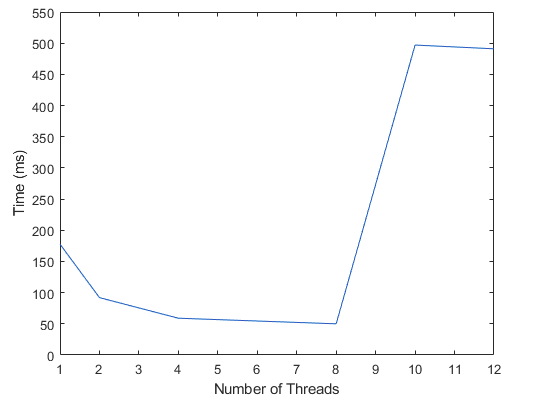
\includegraphics[width=0.97\columnwidth]{Figuras/img5.png}
\caption{Primeira questão.}
\label{stability}
\end{figure}


%%%%%%%%%%%%%%%%%%%%%%%%%%%%%%%%%%%%%%%%%%%%%%%%%%%%%%%%%%%%%%%%%%%%%%%%%%%%%%%%%%%%%%%%%%%%
\section{Activity 2: Matrix-Vector Product }
1. The matrix-vector product for an mxn matrix can be computed as

\begin{equation*}
\begin{bmatrix} 
a_{00} &a_{01} & \cdots & a_{0n}\\ a_{10} & a_{11} & \cdots & a_{1n}\\ \vdots & \vdots & & \vdots\\ a_{m0} & a_{m1} & \cdots & a_{mn}\end{bmatrix} \begin{bmatrix}b_{0}\\ b_{1}\\ \vdots\\ b_{n}\end{bmatrix}=\begin{bmatrix} a_{00}b_{0}+a_{01}b_{1}+ \cdots +a_{0n}b_{n}\\ a_{10}b_{0}+a_{11}b_{1}+ \cdots +a_{1n}b_{n}\\ \vdots\\ a_{m0}b_{0}+a_{m1}b_{1}+\cdots+a_{mn}b_{n}
\end{bmatrix}. 
\end{equation*}

2. This can be interpreted as a series of dot products. Modify the dot product code from Activity 1 to compute a 
matrix-vector product.
\newline
\newline
A multiplicação de matrizes é definida pela multiplicação das linhas da primeira vezes a coluna da segunda, e somando em seguida. Desde que o número de coluna da primeira seja igual ao número de coluna da segunda. 
O algoritmo que define a operação é dado como, o código abaixo, note que não é um código ótimo.
\newpage
\begin{scriptsize}
\estiloR
\begin{lstlisting}[caption={Código fonte referente a segunda questão.}, label=lst:rcode]

#include <pthread.h>
#include <omp.h>
#include <stdio.h>
#include <stdlib.h>

#define N 500
#define NUMTHREADS 64

int A[N][N];
int B[N][N];
int C[N][N];

int main(int argc, char* argv[]) 
{
    int i,j,k;
    for (i= 0; i< N; i++){
        for (j= 0; j< N; j++){
            A[i][j] = 2;
            B[i][j] = 2;
         }       
    }

    double time= - omp_get_wtime();
    #pragma omp parallel for private(i,j,k)
    #shared(A,B,C) num_threads(NUMTHREADS)
    for (i = 0; i < N; ++i) {
        for (j = 0; j < N; ++j) {
            for (k = 0; k < N; ++k) {
                C[i][j] += A[i][k] * B[k][j];
            }
        }
    }

    time+=omp_get_wtime();
    printf("%f segundos \n",time);

}

\end{lstlisting}
\end{scriptsize}
3. Parallelize this matrix-vector product and perform an analysis on the execution time versus number of threads for 
several different matrix dimension
\begin{table}[!h]
%\centering
\begin{tabular}{|c|c|c|}
\hline
	Número de Threads & Tempo (s) & N-colunas/N-linhas \\
	\hline\hline
	1 & 6.680 & 1000\\
	\hline
    2 & 5.087 & 1000\\
    \hline
    4 & 4.897 & 1000\\
    \hline
    8 & 4.72 & 1000\\
    \hline
    10 & 4.680 & 1000\\
    \hline
    12 & 4.800 & 1000\\
\hline
\end{tabular}
\end{table}
\begin{table}[!h]
%\centering
\begin{tabular}{|c|c|c|}
\hline
	Número de Threads & Tempo em segundos \\
	\hline\hline
	1 & 0.639 & 500\\
	\hline
    2 & 0.419 & 500\\
    \hline
    4 & 0.380 & 500\\
    \hline
    8 & 0.304 & 500\\
    \hline
    10 & 0.298 & 500\\
    \hline
    12 & 0.305 & 500\\
\hline
\end{tabular}
\end{table}

Analisando os gráficos bem como suas tabelas notamos um crescimento substancial no processamento das matrizes em relação aos tempos de execução quando comparamos o uso de matrizes de 500x500 e 1000x1000. Mesmo assim notamos que uma semelhança comportamental no processo, o que já era esperado uma vez que a paralelização funciona gradativamente igual ao crescimento do número de instruções.

\begin{figure}[htbp]
\centering
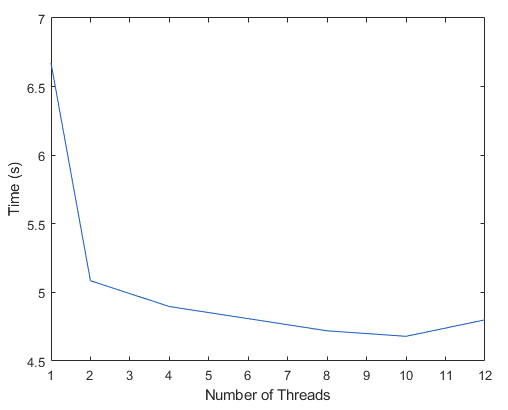
\includegraphics[width=0.97\columnwidth]{Figuras/img6.png}
\caption{Segunda questão.}
\label{stability}
\end{figure}

\begin{figure}[htbp]
\centering
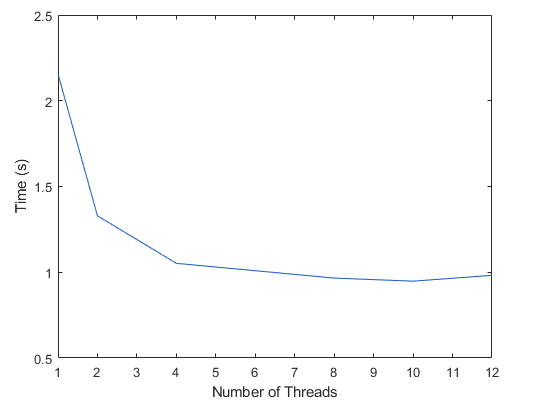
\includegraphics[width=0.97\columnwidth]{Figuras/img4.png}
\caption{Segunda questão.}
\label{stability}
\end{figure}


%%%%%%%%%%%%%%%%%%%%%%%%%%%%%%%%%%%%%%%%%%%%%%%%%%%%%%%%%%%%%%%%%%%%%%%%%%%%%%%%%%%%%%%%%%%%%%%%%

\section{Activity 3: Derivation of the Backward Difference Formula}
Com as fórmulas trabalhadas na seção “Finite Difference Approximation”, foi reproduzida a solução exposta “Foward-Time, Centered Space”. Esta, consiste no desenvolvimento de um esquema discreto capaz de resolver a equação do calor.

\begin{equation*} \phi_{i+1}-\phi_{i-1}=2\Delta x\left.\frac{\partial\phi}{\partial x}\right\vert_{x_{i}}-\frac{2\Delta x^{3}}{3!}\left.\frac{\partial^{3}\phi}{\partial x^{3}}\right\vert_{x_{i}}+\ldots\ ,\tag{4} \end{equation*}

No esquema, define-se a grade que contém pontos em ambos espaço e tempo. Sobre a equação, é dada a aproximação da derivada de primeira ordem no tempo, dependente apenas do ponto atual da grade,  Em seguida, aproximação da derivada de segunda ordem no espaço. Levando os ajustes à equação original, é possível finalmente, atualizar as grades a partir de cada passo atual para o seguinte tendo-a na seguinte forma:

\newpage
\begin{scriptsize}
\estiloR
\begin{lstlisting}[caption={Código referente a quarta questão}, label=lst:rcode]
#include <pthread.h>
#include <omp.h>
#include <stdio.h>
#include <stdlib.h>
#define VECLEN 9999999
#define NUMTHREADS 16

int main (int argc, char* argv[]){
int i, tid, len=VECLEN, threads=NUMTHREADS;
double *a, *b;
double sum, psum;

/* Assign storage for dot product vectors */
a = (double*) malloc (len*threads*sizeof(double));
b = (double*) malloc (len*threads*sizeof(double));
 
for (i=0; i<len*threads; i++) {
  a[i]=1.0;
  b[i]=a[i];
  }
sum = 0.0;

double time= - omp_get_wtime();
#pragma omp parallel 
#private(i,tid,psum) num_threads(threads) 
{
psum = 0.0;
tid = omp_get_thread_num();

#pragma omp for reduction(+:sum)
  for (i=0; i<len*threads; i++) 
    {
    	//printf("\n%d\n", omp_get_wtime());
      sum += (a[i] * b[i]);
      psum = sum;
    }

time+=omp_get_wtime();
printf("%f segundos \n",time);

free (a);
free (b);
}   

\end{lstlisting}
\end{scriptsize}

\section{Activity 4:FTCS Test Problem}
1. As a test problem, start with the initial condition
\begin{equation*} \phi(x, 0)=\sin\left(\frac{\pi x}{L}\right), \end{equation*}

with boundary conditions x0=xL=0 K. Use the parameters L=1 m,Δt=5×10−5 s, Δx=10−2m, and tmax=0.5 s. This set will give r≈0.49, which is below the stability threshold.

2. Create a plot showing the approximate solution at different times up to tmax.

3. The exact solution to Equation 1 with the boundary and initial conditions above is given by

\begin{equation*} \phi(x, t)=\sin\left(\frac{\pi x}{L}\right)\exp\left(-\frac{\alpha\pi^{2}t}{L^{2}}\right). \end{equation*}

Confirm that the FTCS solution at tmax is approximately the same as the exact solution. \\

Choose values for Δt,Δx, and α that give a value of r>0.5. Create the same plot as above. Depending on the chosen parameters, the instability in the FTCS scheme will be seen as an oscillation in the solution curve. \\
\begin{scriptsize}
\estiloR
\begin{lstlisting}[caption={Código em MATLAB referente a terceira questão.}, label=lst:rcode]
(nt,nx,alpha)
\end{lstlisting}
\end{scriptsize}

\begin{figure}[htbp]
\centering
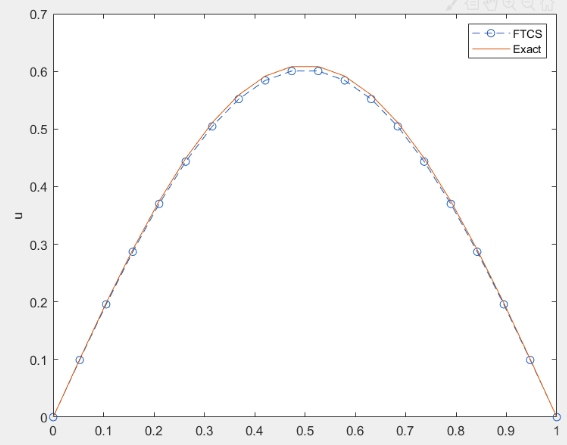
\includegraphics[width=0.97\columnwidth]{Figuras/mat1.png}
\caption{(10,20,0.1).}
\label{stability}
\end{figure}
\begin{figure}[htbp]
\centering
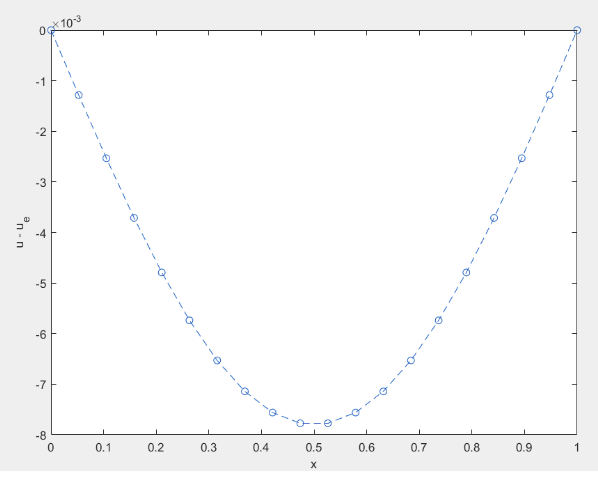
\includegraphics[width=0.97\columnwidth]{Figuras/mat2.png}
\caption{Estimativa de erro entre as previsões.}
\label{stability}
\end{figure}
\begin{figure}[htbp]
\centering
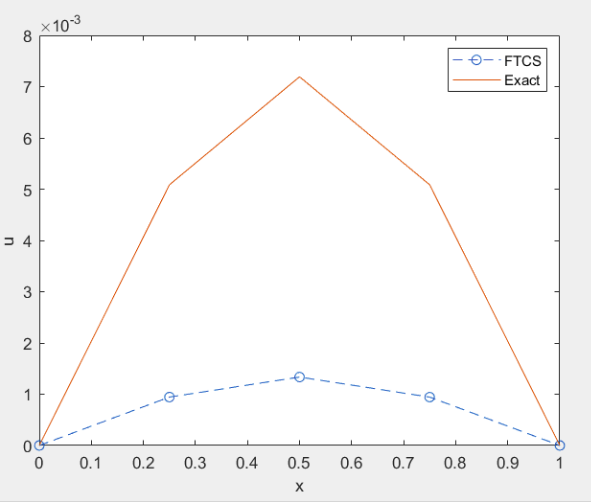
\includegraphics[width=0.97\columnwidth]{Figuras/mat3.png}
\caption{(10,5,1).}
\label{stability}
\end{figure}
\begin{figure}[htbp]
\centering
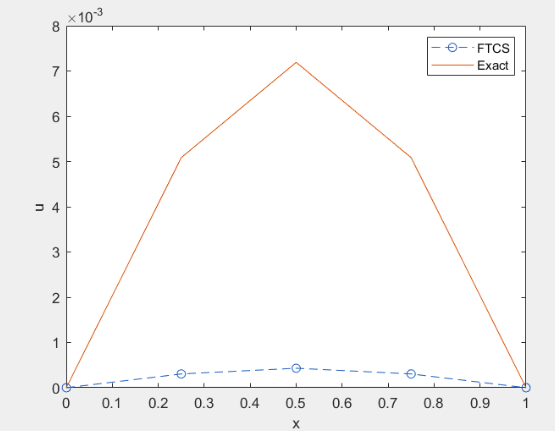
\includegraphics[width=0.97\columnwidth]{Figuras/mat4.png}
\caption{(8,5,1).}
\label{stability}
\end{figure}
\begin{figure}[htbp]
\centering
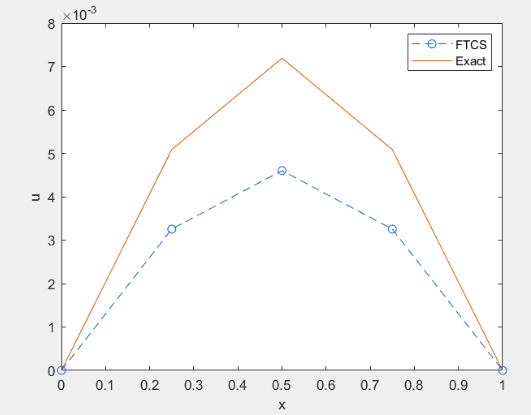
\includegraphics[width=0.97\columnwidth]{Figuras/mat5.png}
\caption{(20,5,1).}
\label{stability}
\end{figure}

%%%%%%%%%%%%%%%%%%%%%%%%%%%%%%%%%%%%%%%%%%%%%%%%%%%%%%%%%%%%%%%%%%%%%%%%%%%%%%%%%%%%

\section{Activity 5: FTCS Parallelization }
1. Use the same test problem as Activity 4. Parallelize the spatial loop using the #pragma omp for directive. In addition, 
add calls to omp\_get\_wtime() so that you can compute the elapsed time of the program, specifically the loop over time. 
Adjust the parameters so that you are below the stability threshold and the calculation takes approximately 10 seconds. 

\newpage
\begin{scriptsize}
\estiloR
\begin{lstlisting}[caption={Código referente a quinta questão}, label=lst:rcode]
#include <pthread.h>
#include <omp.h>
#include <stdio.h>
#include <stdlib.h>
#include <math.h>

#define NUMTHREADS 8
#define PI 3.14159265358979323846
int main(){

	int nt = 10;
	int nx = 20; 
	float alpha = 0.1; 
	int L = 1; 
	float tmax = 0.5; 
	int errPlots=1; 
	float dx=L/(nx-1);
	float dt = tmax/(nt-1);
	float r = alpha*dt/(dx*dx); 
	float r2 = 1 - 2*r;
	float x[20];
	float t[10];
	float U[20][10] = {0};
	int i;
	for (i=0; i<20; i++){
		x[i] = i*0.0526;
	}

	for (i=0; i<10; i++){
		t[i] = i*0.0556;
	}

	for (i=0; i<20; i++){
		U[i][0] = sin(PI*x[i]/L);

	}
	int u0 = 0, uL = 0;

	double time= - omp_get_wtime();
	int m;
	#pragma omp parallel for private(i,m).
	#shared(U) num_threads(NUMTHREADS)
    for (m=1; m<nt; m++){
    	for (i=1; i<nx-1; i++){
    		#pragma omp critical
    			 U[i][m] = r*U[i-1][m-1] 
    			 + r2*U[i][m-1] + r*U[i+1][m-1];
       
    	}
	}
    time+=omp_get_wtime();
    printf("%f segundos \n",time);

}


\end{lstlisting}
\end{scriptsize}

2. Verify that after parallelization you obtain the same results as the serial version. 
\begin{table}[!h]
%\centering
\begin{tabular}{|c|c|c|}
\hline
	Número de Threads & Tempo em segundos \\
	\hline\hline
	1 & 6.730\\
	\hline
    2 & 6.880\\
    \hline
    4 & 6.980\\
    \hline
    8 & 6.620\\
    \hline
    10 & 4.580\\
\hline
\end{tabular}
\end{table}

\begin{figure}[htbp]
\centering
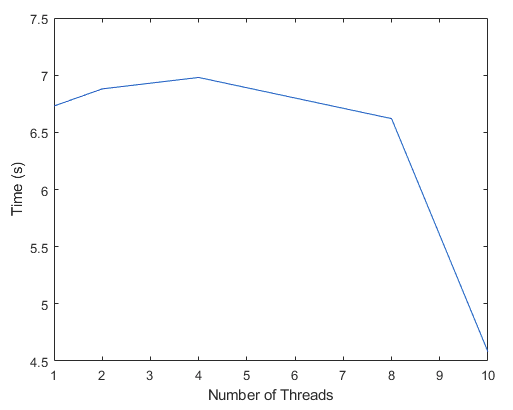
\includegraphics[width=0.97\columnwidth]{Figuras/img7.png}
\caption{(20,5,1).}
\label{stability}
\end{figure}
3. Perform a strong scaling analysis on the code, that is, compute the runtime for a variety of threads, even beyond the 
number available on your system and plot the execution time versus the number of threads. 
The look of the strong scaling analysis will vary depending on the specifications of the system used to do the calculation.
As an example, Figure 5 shows the strong scaling on a six-core Intel Xeon processor for up to 12 threads. Most small 
applications will scale relatively well up to the number of cores on the system. Beyond that, the performance tends to 
flatten or get worse, mainly due to more threads attempting to use the same limited resources




%%%%%%%%%%%%%%%%%%%%%%%%%%%%%%%%%%%%%%%%%%%%%%%%%%%%%%%%%%%%%%%%%%%%%%%%%%%%%%%%
\section{Conclusions}
O procedimento de modelagem proposto torna possível o entendimento e o detalhamento do sistema produtivo de modo progressivo, através de refinamentos sucessivos. A abordagem adotada permite uma melhor caracterização dos elementos do sistema e do relacionamento entre eles. Um modelo relativamente simples pode representar elementos que possuem características comuns, garantindo a sua reusabilidade, isto é, uma biblioteca de modelos pode ser implementada. Em suma concluímos como é notável a melhora de desempenho com a paralelização. 


\section{Source Code}

Os códigos aqui citados estão disponíveis em: \url{\GitHubLoc}, inclusive bibliotecas e tutoriais para desenvolvimento de 
tecnologias ligadas a modelagem e simulação de eventos naturais.

%%%%%%%%%%%%%%%%%%%%%%%%%%%%%%%%%%%%%%%%%%%%%%%%%%%%%%%%%%%%%%%%%%%%%%%%%%%%%%%%

\bibliographystyle{ieeetr}
\bibliography{bibliografia}

\section{Agradecimentos}

Meus pais, minha noiva, amigos e ao laboratório laccan-UFAL.

\clearpage

\end{document}
